\documentclass{article}

\usepackage[margin=1in]{geometry}
\usepackage{listings}
\usepackage{color}
\usepackage{graphicx}
\usepackage{float}

\title{Lab 5: Timer and PWM Operations}
\date{October 31, 2017}
\author{Matthew Friedman 861151348\\Souradeep Bhattacharya 861105938\\EE128 Section: 021}

\definecolor{dkgreen}{rgb}{0,0.6,0}
\definecolor{gray}{rgb}{0.5,0.5,0.5}
\definecolor{mauve}{rgb}{0.58,0,0.82}

\lstset{frame=tb,
	language=C,
	aboveskip=3mm,
	belowskip=3mm,
	showstringspaces=false,
	columns=flexible,
	basicstyle={\small\ttfamily},
	numbers=left,
	numberstyle=\color{gray},
	keywordstyle=\color{blue},
	commentstyle=\color{dkgreen},
	stringstyle=\color{mauve},
	breaklines=true,
	breakatwhitespace=true,
	tabsize=4
}

\begin{document}
	\maketitle
	\section*{Abstract}
	The objective of this lab is to program timer operations and pulse-width modulation techniques on the Dragon and Arduino boards. In this lab we created a program that would detect the duty cycle of a PWM signal and then write that to a bi-decade 7-segment display.
	\section*{Experimental System Specification}
	In this lab we built a system that would detect and display the duty cycle of the PWM output of an Arduino.
	\section*{Block Diagram}
	\begin{figure}[H]
		\centering
		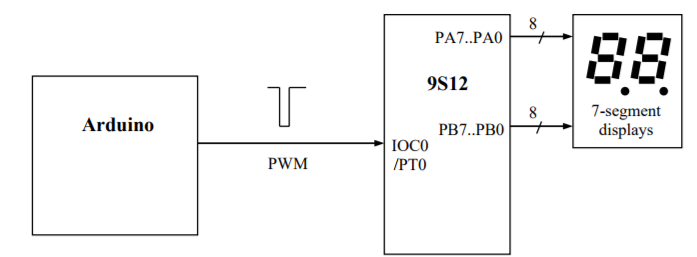
\includegraphics[width=1\textwidth]{Block_Diagram}
	\end{figure}
	\section*{Detailed Schematic}
	\begin{figure}[H]
		\centering
		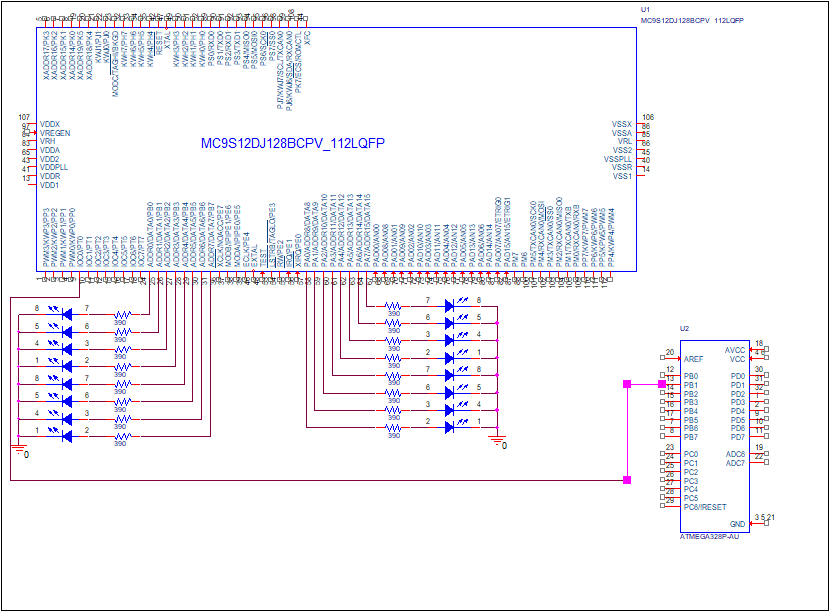
\includegraphics[width=1\textwidth]{Diagram}
	\end{figure}
	\section*{High Level Description of Software}
	We looked at the duty cycle and determined the percent uptime, then we looked to find the total cycle time and calculated the percent uptime. We then displayed this on the bi decade 7 segment display. 
	\section*{Program Listing}
	\subsection*{Dragonboard code}
	\begin{lstlisting}
	#include <hidef.h>
	#include <stdio.h>
	#include <mc9s12dg256.h>
	
	//setup variables
	unsigned long t1, t2, t3, diff, overflow, i;
	unsigned long pulse_width;
	unsigned char decoder[10] = {0x7E, 0x30, 0x6D, 0x79, 0x33, 0x5B, 0x5F, 0x70, 0x7F, 0x7B};
	float raw_pwm = 0.0;
	unsigned char ones = 0;
	unsigned char tens = 0;
	
	//define ISR function
	__interrupt void tovf_isr(void)
	{
	TFLG2 = 0x80; /* clear TOF flag */
	overflow = overflow + 1;
	}
	
	//declare ISR prototype
	typedef void (*near tIsrFunc)(void);
	const tIsrFunc _ovfVect @0x3E5E = tovf_isr; /* register ISR */
	
	void main(void)
	{
		do
		{  
		
		//setup ports
		DDRA = 0xFF; //7seg tens
		DDRB = 0xFF; //7seg ones
		
		//set registers to rising edge
		overflow = 0;
		TSCR1 = 0x80; /* enable timer */
		TSCR2 = 0x05; /* set prescaler to 32 */
		TIOS &= ~0x01; /* select input-capture 0 */
		TCTL4 = 0x01; /* prepare to capture the rising edge */
		TFLG1 = 0x01; /* clear C0F flag */
		
		//capture the rising edge
		while(!(TFLG1 & 0x01)); /* wait for the arrival of the rising edge */
		t1 = TC0; /* save the first edge */
		TFLG1 = 0x01; /* clear C0F flag */
		TFLG2 = 0x80; /* clear TOF flag */
		TSCR2 |= 0x80; /* enable TCNT overflow interrupt */
		EnableInterrupts;
		
		//set registers to falling edge
		TCTL4 = 0x02; /* prepare to capture the falling edge */
		while (!(TFLG1 & 0x01)); /* wait for the arrival of the falling edge */
		t2 = TC0; /* save the second edge */
		TFLG1 = 0x01; /* clear C0F flag */
		TFLG2 = 0x80; /* clear TOF flag */
		TCTL4 = 0x01; /* prepare to capture the rising edge */
		
		//capture the next rising edge
		while(!(TFLG1 & 0x01)); /* wait for the arrival of the rising edge */
		t3 = TC0; /* save the next edge */
		
		//calculate the duty cycle
		if (t2 < t1) 
		{
			overflow -= 1;
		}
		pulse_width = overflow * 65536u + (t2 - t1); //number of increments from prescaled bus clock
		
		//calculate the percentage duty cycle
		raw_pwm = (float)pulse_width / ((float)t3 - (float)t1);
		tens = raw_pwm*10;
		ones = raw_pwm*100 - tens*10;
		
		PORTA = decoder[tens];//tens
		PORTB = decoder[ones];//ones
		
		for(i = 0; i < 1000000; i++);
		
		}while(1);
	}
	\end{lstlisting}
	\subsection*{Arduino Code}
	\begin{lstlisting}
	/*
	Fading
	
	This example shows how to fade an LED using the analogWrite() function.
	
	The circuit:
	- LED attached from digital pin 9 to ground.
	
	created 1 Nov 2008
	by David A. Mellis
	modified 30 Aug 2011
	by Tom Igoe
	
	This example code is in the public domain.
	
	http://www.arduino.cc/en/Tutorial/Fading
	*/
	
	int ledPin = 5;    // LED connected to digital pin 9
	
	void setup() {
		TCCR0B = (TCCR0B & 0b11111000) | 0x04;
		// nothing happens in setup
	}
		
	void loop() {
		// fade in from min to max in increments of 5 points:
		for (int fadeValue = 0 ; fadeValue <= 255; fadeValue += 5) {
			// sets the value (range from 0 to 255):
			analogWrite(ledPin, fadeValue);
			// wait for 30 milliseconds to see the dimming effect
			delay(200);
		}
		
		// fade out from max to min in increments of 5 points:
		for (int fadeValue = 255 ; fadeValue >= 0; fadeValue -= 5) {
			// sets the value (range from 0 to 255):
			analogWrite(ledPin, fadeValue);
			// wait for 30 milliseconds to see the dimming effect
			delay(200);
		}
	}
	\end{lstlisting}
	\section*{Technical Problems}\
	\paragraph*{Program would not upload} For a while our program would not load on the microcontroller. This was because we had the PWM pin connected to the E1 pin. Once we disconnected it it would load.
	\paragraph*{Could not detect rising edge} Our program could not detect the rising edge. We realized that our program was looking for interrupts on the T0 pin and we had the PWM connected to E1 pin. Once we connected it to the proper pin the program worked as expected.
	\section*{Answers to Question}
	\subsection*{Prelab}
	Uptime is 0.612mS and downtime is 1.429mS.
	\subsection*{Lab Questions}
	\begin{enumerate}
		\item Once the LED was running at 30Hz we could notice it if we paid close attention.
		\item We use the prescaler 32. If we decrease it we can detect events that happen closer in time and if we increase it we can detect events over a longer period of time. In effect it controls the resolution of each bit of the counter variable.
	\end{enumerate}
	\section*{Conclusion}
	In this lab we built a program that could detect the duty cycle of a PWM signal provided by another device. We this displayed this on a bi-decade 7 segment display.
	
\end{document}